\chapter{Web of Data: I Linguaggi}

\section{Introduzione}

\subsection{Perché Studiare il Semantic Web e Linked Data?}

\begin{itemize}
  \item Gli approcci quantitativi non sono sufficienti per domini complessi: 
    \begin{itemize}
      \item Non è possibile apprendere il comportamento giusto per ogni contesto. 
      \item Reattività e ragionamento.
    \end{itemize}
  \item L'ambito della conoscenza è intrinsecamente basato su modelli: 
    \begin{itemize}
      \item Arte, media, tecnologie, etc. 
    \end{itemize}
  \item Interoperabilità dei dati: 
    \begin{itemize}
      \item Conoscenza esperta per stabilire i \fancyglitter{mapping}. 
      \item Utilizzo di standard.
    \end{itemize}
  \item Ruolo nel ragionamento in molte applicazioni: 
    \begin{itemize}
      \item Elaborazione del linguaggio naturale. 
      \item Question answering. 
      \item Chatbots.
    \end{itemize}
\end{itemize}

\subsection{Obiettivi del Corso}

\begin{itemize}
  \item Imparare a rappresentare un dominio di conoscenza con i linguaggi
del Web Semantico (RDF e OWL), che permettono di implementare
ontologie computazionali. 
\item Utilizzare strumenti di ragionamento automatico per realizzare
inferenze sulla conoscenza formalizzata nelle ontologie
computazionali. 
\item Interrogare basi di conoscenza in cui i dati sono rappresentati in un
formato semantico utilizzando il linguaggio SPARQL. 
\item Rendere interoperabili rappresentazioni diverse (ontologie, basi di
dati, fogli di calcolo) utilizzando strumenti di mapping.
\end{itemize}

\section{Dalle Reti Semantiche alle Ontologie}

\subsection{I Limiti della Logica Classica}

A partire dagli anni 60 si è sviluppata una branca
dell’intelligenza artificiale specificamente orientata alla
rappresentazione della conoscenza. Questo rappresenta un tentativo di superare la logica classica allora utilizzata. Il motivo è che la logica classica ha alcuni limiti importanti: 

\begin{itemize}
  \item È caratterizzata da \fancyglitter{inadeguatezza espressiva}.
  \item È \fancyglitter{monotòna}. 
  \item Presenta svantaggi dal punto di vista \fancyglitter{computazionale}.
\end{itemize}

\dfn{Inadeguatezza Espressiva}{
  Alcuni aspetti dell’inadeguatezza della logica classica possono essere
attribuite a differenze con i sistemi cognitivi. 
}

\clm{}{}{
  \begin{itemize}
    \item La logica classica è un \fancyglitter{formalismo piatto}:
      \begin{itemize}
        \item Tutte le affermazioni si collocano sullo stesso piano. 
        \item Esprime conoscenza di carattere generale e immutabile.
      \end{itemize}
    \item Le procedure di dimostrazione sono diverse dal ragionamento umano\footnote{Da premesse false discendono conseguenze vere.}. 
    \item I \fancyglitter{valori di verità} non sono adatti a rappresentare gli aspetti quantitativi
che caratterizzano il mondo reale
  \end{itemize}
}

\dfn{Monotònicità}{
  La logica del primordine è monotòna: le conoscenze inserite
nel sistema logico non possono essere cancellate.
}

\nt{La conoscenza può solo aumentare.}

\clm{}{}{
  \begin{itemize}
    \item Le nuove conoscenze non possono contraddire quelle già
presenti nel sistema. 
\item Impossibilità di rappresentare il cambiamento, quindi gli
aspetti temporali della conoscenza.
  \end{itemize}
}

\dfn{Limitazioni Computazionali}{
  Il calcolo dei predicati è \newfancyglitter{semi-decidibile}: è possibile
dimostrare con certezza cosa discende dalla base di
conoscenza, ma non si ha la certezza di dimostrare ciò che non discende dalla base di conoscenza.
}

\cor{Inefficienza nelle Procedure di Dimostrazione}{
  Per le sue caratteristiche intrinseche (è un formalismo
orientato alla rappresentazione) le procedure di
dimostrazione non sono abbastanza efficienti per le
applicazioni reali.
}

\qs{}{Ma cosa possiamo dire sulle logiche non classiche?}

\paragraph{Le logiche non classiche rilasciano alcune caratteristiche della logica
classica:}
\begin{itemize}
  \item Valori di verità $\Rightarrow$ \fancyglitter{logiche fuzzy}, hanno valori di verità in un intervallo, nascono per superare la rappresentazione binaria dell'informazione.

\begin{figure}[h]
    \centering
    
\includegraphics[scale=0.3]{01/bknb.png}
    \caption{Rappresentazione accurata di una logica fuzzy.}
\end{figure}
\item Conoscenza certa $\Rightarrow$ \fancyglitter{logiche bayesiane}, incorporano il ragionamento probabilistico. 
\item Monotonicità $\Rightarrow$ \fancyglitter{default logics}, belief revision. 
\item Indecidibilità $\Rightarrow$ insiemi decidibili della logica del primordine. 
\item Inefficienza delle dimostrazioni $\Rightarrow$ uso di \fancyglitter{euristiche} nella dimostrazione automatica.
\end{itemize}

\paragraph{Un quadro storico:}

\begin{itemize}
  \item Anni 60s-70s: reti semantiche e frames. 
  \item Anni 70s-80s: logiche non classiche. 
  \item Anni 80s-90s: logiche descrittive. 
  \item Anni 2000s: ontologie computazionali. 
  \item Dal 2010: Linked Data.
\end{itemize}

\subsection{Reti Semantiche}

\dfn{Reti Semantiche}{Le reti semantiche sono:

\begin{itemize}
  \item Basate su una struttura a \newfancyglitter{grafo}. 
  \item I nodi del grafo rappresentano \newfancyglitter{concetti}. 
  \item Gli archi tra i concetti rappresentanole  \newfancyglitter{relazioni tra concetti}.
\end{itemize}
}

\begin{figure}[h]
    \centering
    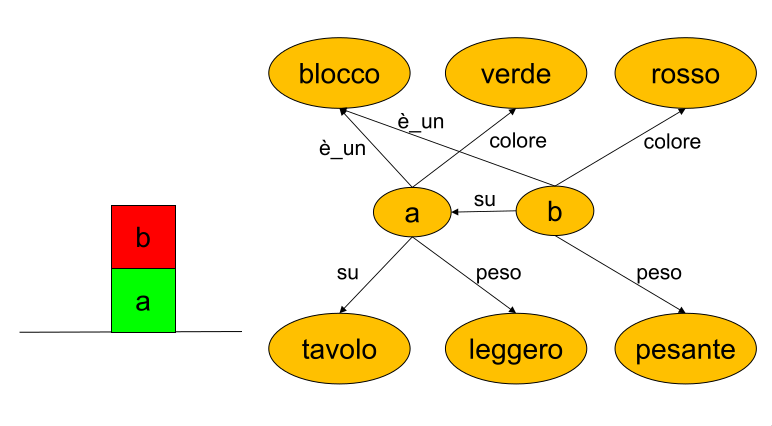
\includegraphics[scale=0.4]{01/grafo.png}
    \caption{Grafo relazionale del "Mondo dei Blocchi", un dominio giocattolo utilizzato nel mondo dell'AI.}
\end{figure}

\nt{Nel "Mondo dei Blocchi" c'è un tavolo su cui è collocato un blocco verde chiamato "a" e sopra un blocco rosso chiamato "b". Una delle possibili rappresentazione è quella dell'immagine in cui sono presenti concetti, qualità ed entità concrete. Gli archi sono varie relazioni.}

\paragraph{Vantaggi di questa rappresentazione:}

\begin{itemize}
  \item Le informazioni relative a un nodo sono \fancyglitter{immediatamente disponibili} dato che ogni blocco è direttamente collegato alle sue proprietà. 
  \item Permette di rappresentare una nozione di \fancyglitter{rilevanza} per cui dato un focus, alcune informazioni si trovano in prossimità. 
\end{itemize}

\paragraph{Corrispondente rappresentazione logica:}

\begin{itemize}
  \item Blocco(a). 
  \item Blocco(b). 
  \item su(b,a). 
  \item su(a,tavolo). 
  \item rosso(b). 
  \item verde(a). 
  \item pesante(b). 
  \item leggero(a).
\end{itemize}

\cor{Ragionamento nelle Reti Semantiche}{
  Nelle reti semantiche il ragionamento consiste nel seguire
un percorso tra nodi.
}

\qs{}{Su quale blocco si trova il blocco b?}

\paragraph{Risposta:} È sufficiente seguire l’arco etichettato come «su» nella rete,
da b verso il nodo a cui punta. Seguendo ulteriormente gli archi si possono inferire relazioni
indirette: il blocco b è "al di sopra" del tavolo.

\subsection{Reti Semantiche e Logica}

L’espressività delle reti semantiche corrisponde a un sottoinsieme della logica del primordine:

\begin{itemize}
  \item Nodi = \fancyglitter{termini}. 
  \item Archi = \fancyglitter{predicati}
\end{itemize}

\begin{figure}[h]
    \centering
    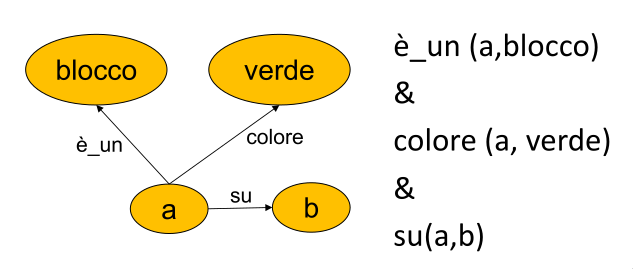
\includegraphics[scale=0.4]{01/grafo2.png}
    \caption{Grafo relazionale in relazionale alla logica del primordine.}
\end{figure}

\nt{Alcune relazioni possono coinvolgere più di due entità.}

\begin{figure}[h]
    \centering
    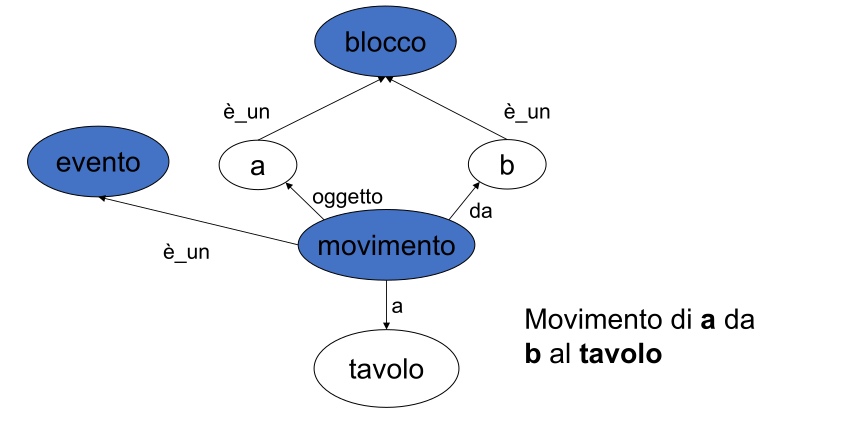
\includegraphics[scale=0.4]{01/grafo3.png}
    \caption{La relazione “movimento” che unisce a, b e tavolo diventa un termine cioè un nodo.}
\end{figure}

\dfn{Reti Semantiche Proposizionali}{
  Le \newfancyglitter{reti semantiche proposizionali} includono nodi che
rappresentano proposizioni. Usando nodi per rappresentare proposizioni è possibile
introdurre una \newfancyglitter{dimensione epistemica}: 
\begin{itemize}
  \item Rappresentare credenze soggettive. 
  \item Lo stesso sistema può rappresentare le credenze di più soggetti
senza che insorgano contraddizioni. 
\end{itemize}
}

\clm{}{}{
  \begin{itemize}
    \item Reti semantiche proposizionali posso avere l’espressività
della logica del primordine una volta introdotti connettivi,
variabili, quantificatori, ecc. 
\item Anche l’inferenza nelle reti proposizionali ha le stesse
caratteristiche che nella logica del primordine. 
\item Soluzione: limitare l’espressività privilegiando tipi di
ragionamento più comuni e computazionalmente trattabili.
  \end{itemize}
}

\dfn{SNePs}{
  Rete semantica proposizionale che incorpora alcuni
elementi della teoria dei frame (Shapiro '79).
}

\nt{Si tratta di una rete semantica con un \fancyglitter{motore di ragionamento}. Permette vari tipi di ragionamento:
\begin{itemize}
  \item Su formule. 
  \item Su slot. 
  \item Su percorsi. 
\end{itemize}
}

\begin{figure}[h]
    \centering
    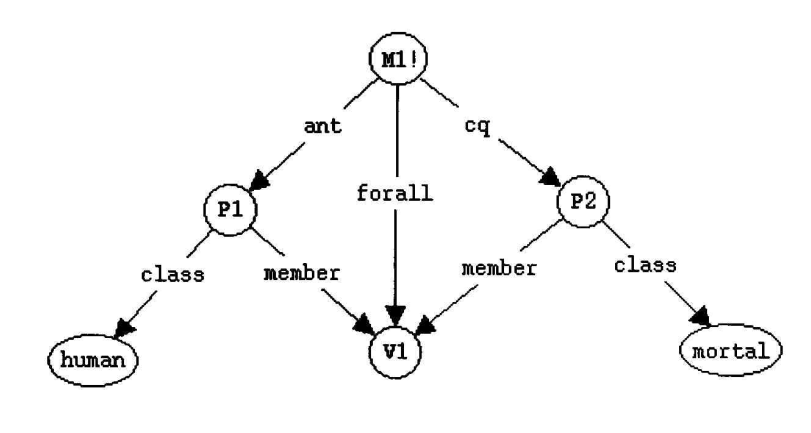
\includegraphics[scale=0.3]{01/socrate.png}
    \caption{Tutti gli uomini sono mortali.}
\end{figure}

\qs{}{Di cosa parla la rete?}

\dfn{Eterogeneità}{
  \begin{itemize}
    \item Archi rappresentano relazioni di tipo diverso tra concetti (relazioni
epistemiche vs fatti). 
\item Nodi rappresentano concetti di tipo diverso (blocco A, blocco)
  \end{itemize}
}

\nt{Alcuni tipi di nodi e di archi sono particolarmente importanti.}

\begin{figure}[h]
    \centering
    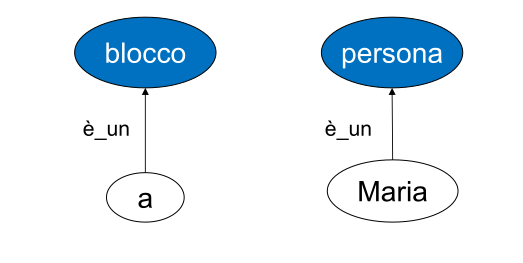
\includegraphics[scale=0.35]{01/node.png}
    \caption{I nodi colorati rappresentano tipi di entità (classi), i nodi bianchi
rappresentano entità singole (individui).}
\end{figure}

\qs{}{"What ISA is and isn't?"}

\begin{itemize}
  \item Gli archi “è un” (IS-A o ISA) hanno un significato diverso
se collegano due classi oppure un individuo a una classe. 
\item Brachman ('83) propone di distinguere i due tipi di
relazioni: “What isa is and isn’t”: 
\begin{itemize}
  \item \fancyglitter{Archi ISA}: appartenenza di una classe a una sottoclasse
(transitiva).
\item \fancyglitter{Archi instance\_of}: appartenenza di un individuo a una classe.
\end{itemize}
\end{itemize}

\begin{figure}[h]
    \centering
    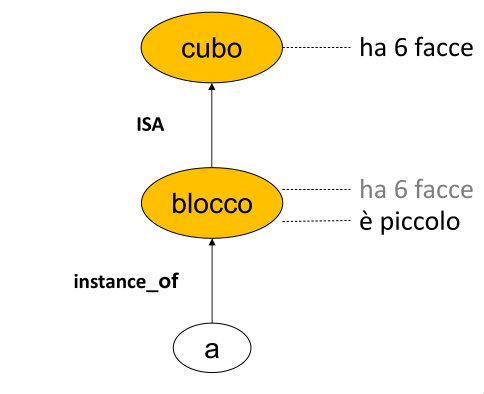
\includegraphics[scale=0.3]{01/ISA.png}
    \caption{ISA e instance\_of.}
\end{figure}

\dfn{Tassonomia}{
  Utilizzando la relazione ISA è possibile esprimere
conoscenza di tipo tassonomico. Si utilizza un ragionamento classificatorio: 
\begin{itemize}
  \item Y è una sottoclasse di Z? $\Rightarrow$ archi ISA. 
  \item x appartiene alla classe Y? $\Rightarrow$ archi instance\_of.
\end{itemize}
}

\begin{figure}[h]
    \centering
    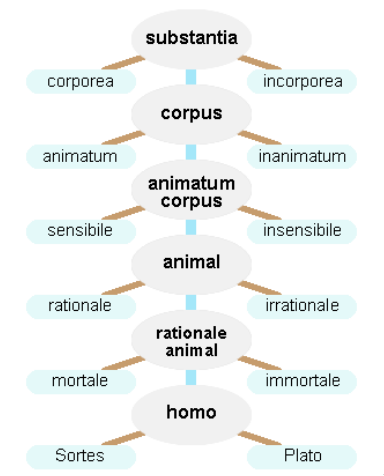
\includegraphics[scale=0.45]{01/porfirio.png}
    \caption{Rappresentazione che deriva dalla filosofia aristotelica, confluita nella scolastica, in cui si raffigurano i principali concetti del pensiero dalla sostanza all'uomo.}
\end{figure}

\nt{Ogni livello \fancyglitter{eredità} le caratteristiche del livello superiore e le caratteristiche non si sovrappongono.}

\paragraph{Vantaggi dell'ereditarietà:}

\begin{itemize}
  \item E’ possibile avere una rappresentazione meno
ridondante facendo una semplice assunzione:
\begin{itemize}
  \item Una classe eredita le proprietà delle classi di cui è sottoclasse. 
  \item Se i cubi hanno sei facce e i dadi sono una sottoclasse dei
cubi, allora anche i dadi hanno sei facce.
\end{itemize}
\item Le sottoclassi hanno proprietà più specifiche delle classi. 
\item Seguendo il percorso degli archi ISA e instance\_of e
diventa possibile ragionare sulle proprietà di un
individuo/classe.
\end{itemize}

\nt{Ma esistono eccezioni, per esempio i pinguini non volano, ma non per questo smettono di essere uccelli. Allo stesso tempo può essere falso per un individuo all'interno di una sottoclasse.}

\dfn{Default Rules}{
  Per gestire le eccezioni è necessario rilasciare la proprietà della
monotonicità (la conoscenza non diminuisce mai). Un esempio è la Default Logic: assunzioni che possono essere
cancellate quando sopravviene nuova conoscenza.
}

\clm{}{}{
  \begin{itemize}
    \item Il trattamento delle eccezioni nelle reti semantiche si basa
sul principio che le conoscenze specificate localmente a un
certo nodo prevalgono su quelle ereditate. 
\item Un corollario è che le conoscenze che comportano meno
passi di inferenza prevalgono su quelle che ne comportano di
più. 
\item Questo principio però non permette di scongiurare tutti gli
inconvenienti.
  \end{itemize}
}

\begin{figure}[h]
    \centering
    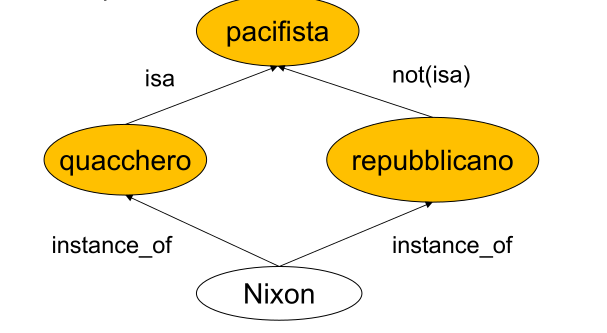
\includegraphics[scale=0.55]{01/nixon.png}
    \caption{Nixon è pacifista o guerrafondaio? In quando quacchero, lo è; in quanto repubblicano,
non lo è (Reiter and Criscuolo, On Interacting Defaults, 1981).}
\end{figure}

\nt{Nemmeno la logica dei default risolve il problema, ciascun default blocca l’altro.}

\dfn{Frame Theory}{
  Evoluzione delle reti semantiche finalizzata a
  rappresentare la conoscenza di tipo stereotipato. Conoscenza di sfondo utile per alcune applicazioni come la \newfancyglitter{visione artificiale} o \newfancyglitter{l’elaborazione del linguaggio}.
}

\dfn{Frame}{
  Un \newfancyglitter{frame} è una struttura dati per la rappresentazione situazioni stereotipate, come trovarsi in una certa tipo di soggiorno o andare al compleanno di un bambino partito. I livelli superiori del telaio sono fissi, e rappresentano cose che sono sempre vere riguardo le situazioni presunte. I livelli inferiori hanno molti terminali: slot che devono essere riempiti da istanze o dati specifici.
}

\cor{Slot}{
  Ogni terminale (slot) può specificare le condizioni che Gli incarichi devono soddisfarsi. (Gli incarichi sono solitamente telai ausiliari più piccoli). Le condizioni possono richiedere un terminale l'incarico di essere una persona, un oggetto ora puntatore a un subframe di un certo tipo. I terminali di un frame sono solitamente riempiti da assegnazioni predefinite. Collezioni di frame collegati sono uniti in frame systems.
}

\paragraph{Struttura di un frame:}

\begin{itemize}
  \item Identificativo. 
  \item Slot: permettono di creare una tassonomia di frame. 
  \item Slot generici: i valori degli slot sono vincolati a un certo tipo, però il contenuto di uno slot può puntare a un altro frame. 
  \item Procedure per il calcolo automatico dei valori. 
  \item Valori predefiniti.
\end{itemize}

\begin{figure}[h]
    \centering
    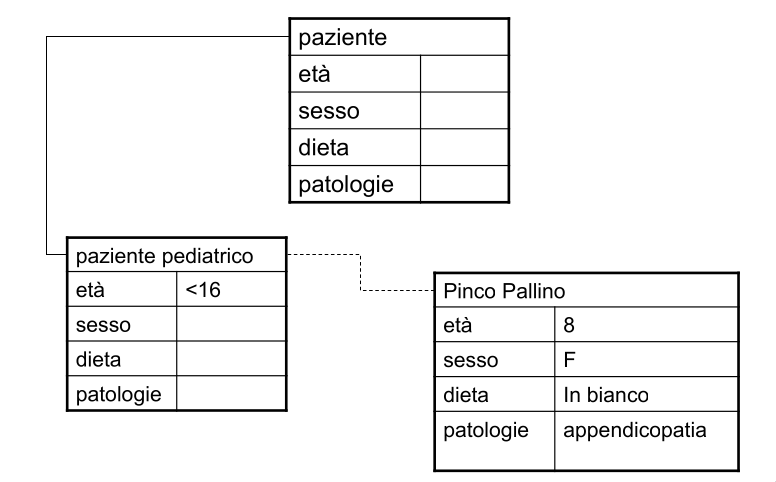
\includegraphics[scale=0.48]{01/tassonomia.png}
    \caption{Esempio di tassonomia.}
\end{figure}

\begin{figure}[h]
    \centering
    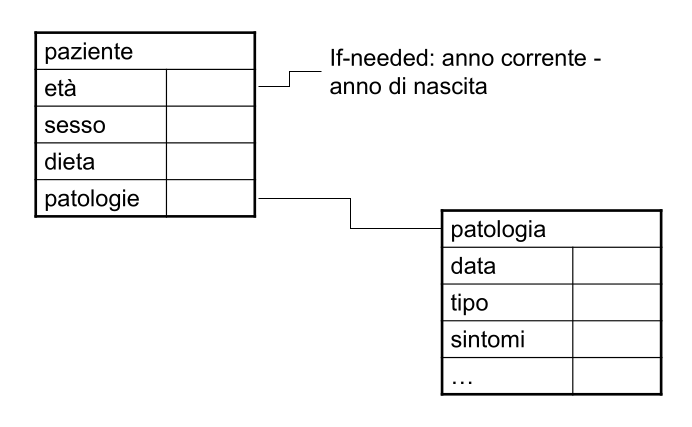
\includegraphics[scale=0.48]{01/non tassonomia.png}
    \caption{Esempio di collegamenti non tassonomici.}
\end{figure}

\dfn{Regole di Produzione}{
  Conoscenza di tipo condizione-azione. Regole IF - THEN (anche dette produzioni): 
  \begin{itemize}
    \item \newfancyglitter{La parte sinistra}: condizioni per l’applicazione delle regola. 
    \item \newfancyglitter{La parte destra}: azioni che sono effettuate se la condizione è
soddisfatta.
  \end{itemize}
}

\clm{}{}{
  \begin{itemize}
    \item Conoscenza dichiarativa: 
      \begin{itemize}
        \item IF allatta(animale,prole) THEN
isa(animale,mammifero). 
\item IF febbre>38,5 and tosse THEN
malattia\_da\_raffreddamento.
      \end{itemize}
    \item Conoscenza procedurale:
      \begin{itemize}
        \item IF intensità(sibilo)>t THEN chiudi(valvola,5mm).
      \end{itemize}
  \end{itemize}
}

\subsection{Sistemi a Regole}

\paragraph{Componenti:}

\begin{itemize}
  \item Base delle regole. 
  \item Memoria di lavoro. 
  \item Interprete delle regole: motore inferenziale. 
\end{itemize}

\paragraph{L'interprete delle regole esegue questo ciclo:}

\begin{enumerate}
  \item Confronto (match) tra fatti (nella memoria di lavoro) e
antecedente delle regole. 
\item Risoluzione di conflitti (più regole applicabili). 
\item Esecuzione (e aggiunta di nuovi fatti alla memoria di lavoro).
\end{enumerate}

\paragraph{Conflitti di applicazione:}

\begin{itemize}
\item \fancyglitter{Refrattarietà}: la stessa regola non viene applicata più volte.
\item \fancyglitter{Recenza}: vengono privilegiate le regole che si applicano ai fatti
più recenti. 
\item \fancyglitter{Specificità}: vengono applicate le regole più specifiche.
\item \fancyglitter{Pesatura}: assegnamento di importanza (peso) a priori alle regole
o ai fatti.
\end{itemize}

\nt{Un passo delicato è il confronto tra la memoria di lavoro e l'antecedente di tutte le regole,}

\dfn{Mycin}{
  Sistema esperto sviluppato a Stanford nei primi anni 70s
(Shortliffe, '75). I fatti sono associati alle probabilità.
}

\begin{figure}[h]
    \centering
    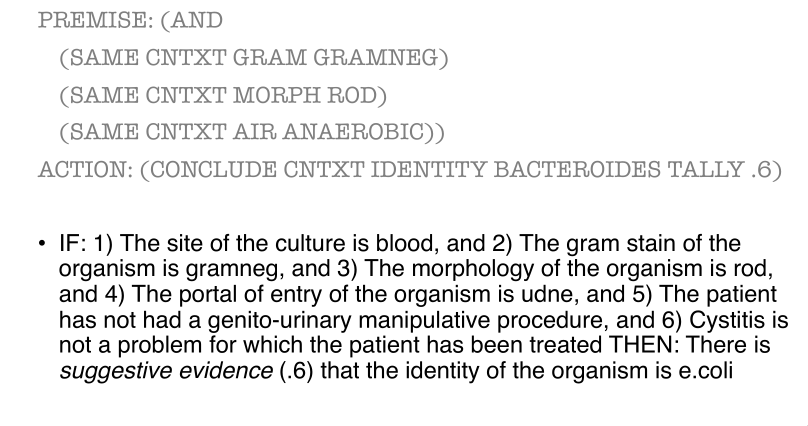
\includegraphics[scale=0.4]{01/mycin.png}
    \caption{Esempio di Mycin.}
\end{figure}

\section{Il Sistema SNePS}

SNePs è una rete semantica e sistema proposizionale che supporta vari tipi di inferenza. 

\begin{figure}[h]
    \centering
    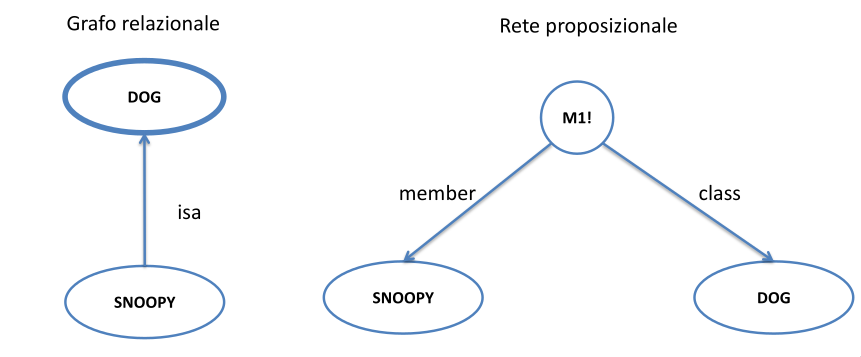
\includegraphics[scale=0.4]{01/SNePS.png}
    \caption{Nella rappresentazione di SNwPS (a destra) la proposizione “Snoopy
è un cane” è rappresentata da un nodo (M1!).
Nessun arco denota una proposizione x isa (è un) y, come invece
avviene nel grafo relazionale (a sinistra).}
\end{figure}

\clm{}{}{
  \begin{itemize}
  \item SNePS fu progettato per la \fancyglitter{robotica cognitiva}. 
    \item Solo i nodi sono espressioni ben formate dotate di una
semantica. 
\item Ogni nodo denota un’\fancyglitter{entità mentale}.
  \end{itemize}
}

\paragraph{Il sistema SNePS è un software dotato delle
seguenti funzionalità:}

\begin{itemize}
  \item Rappresentare la rete: si utilizza un linguaggio utente
    fatto di comandi che permettono di \fancyglitter{fare asserzioni}
    (Socrate è un uomo), \fancyglitter{esprimere regole} (Gli uomini
    sono mortali) e \fancyglitter{manipolare la rete} (creare
proposizioni non asserite). 
\item \fancyglitter{Cercare} nella rete nodi con certe caratteristiche (gli
individui che sono uomini). 
\item \fancyglitter{Inferire} nuove asserzioni a partire da quelle esistenti.
\end{itemize}

\paragraph{Input e Output:}

\begin{itemize}
  \item L'utente usa il \fancyglitter{linguaggio utente} per asserire una proposizione.
  \item Il sistema crea una rete che rappresenta la proposizione: 
    \begin{itemize}
      \item Tipicamente, un nodo “proposizione” da cui emanano degli archi. 
      \item La rappresentazione viene creata internamente al sistema e
comunicata all’utente per mezzo di una particolare notazione
(\fancyglitter{linguaggio del sistema}). 
\item Alcune versioni del sistema erano dotate di un output grafico per
rappresentare visivamente la rete. 
    \end{itemize}
  \item Un insieme di proposizioni può essere interrogata oppure può
diventare la base per inferenze. Sia l’estrazione di proposizioni dalla rete che la deduzione di nuove
proposizioni avvengono su richiesta dell’utente, cioè quando l’utente
digita il comando corrispondente nel linguaggio utente. 
\end{itemize}


\paragraph{Tipi di nodo:}

\begin{itemize}
  \item I nodi molecolari (M$i$) hanno archi uscenti.
Rappresentano proposizioni, incluse le regole di
ragionamento, oppure individui. 
\item I nodi base (B$i$) non hanno archi uscenti.
Rappresentano individui che hanno certe
caratteristiche, ma a cui non vogliamo dare un nome. 
\item I nodi variabili non hanno archi uscenti ma
rappresentano individui arbitrari o proposizioni, come
le variabili logiche. 
\end{itemize}

\dfn{Relazioni}{
  Le relazioni tra i nodi sono date dagli archi che li
uniscono. Se non specificato diversamente una relazione tra
un nodo A e uno B genera un arco diretto da A
verso B con il nome della relazione specificata. 
}

\nt{
  Il comando seguente definisce due relazioni, isa e
ako (a kind of):
\begin{center}
 (define isa ako) 
\end{center}

}

\begin{figure}[h]
    \centering
    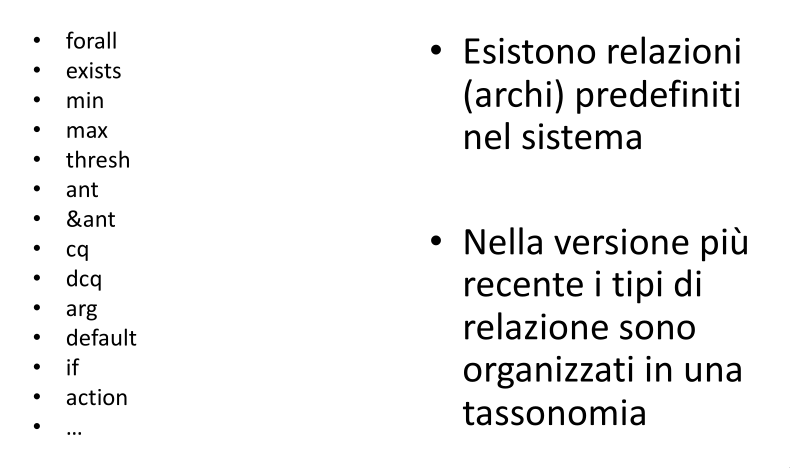
\includegraphics[scale=0.4]{01/rel.png}
    \caption{Alcune relazioni predefinite.}
\end{figure}

\dfn{Asserzione}{
  Il comando \newfancyglitter{assert} permette di asserire una proposizione. 
  Ha come argomento una lista di coppie, di cui: 
  \begin{itemize}
    \item Il primo elemento è una relazione. 
    \item Il secondo è un node o una lista di nodi.
  \end{itemize}
}

\ex{Assert}{
  \begin{center}
    (assert member Clyde class elephant)
  \end{center}
  Il sistema costruirà un nodo M1 con un arco member
che punta all’identificativo Clyde e un arco class che
punta un nodo elefante. M1! Significa che il nodo M1 è asserito.

\begin{center}
  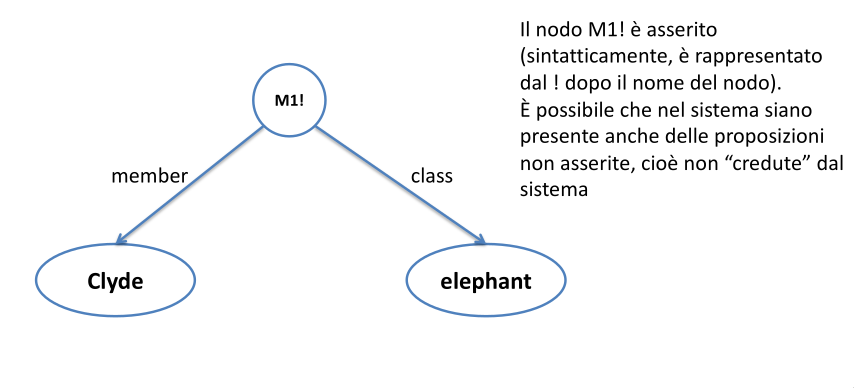
\includegraphics[scale=0.45]{01/clide.png}
\end{center}

}

\dfn{Contesti}{
  Un nodo può essere asserito oppure non asserito. Allo scopo di rappresentare le credenze di più soggetti diversi, il sistema può contenere più
\newfancyglitter{contesti}: 
\begin{itemize}
  \item Un contesto è formato da ipotesi. 
  \item Un’\newfancyglitter{ipotesi} in un contesto è un nodo asserito oppure
derivato via inferenza.
\end{itemize}
}

\nt{Un contesto si crea con il comando: 
\begin{center}
  :context nodeset context-name
\end{center}
}

\paragraph{Uso dei nodi di base:}

\begin{itemize}
  \item I nodi base vengono usati per rappresentare
individui che soddisfano determinate descrizioni
senza dargli un nome. 
\item Non hanno archi uscenti; cioè non hanno
informazioni strutturali. Tutto ciò che si sa di loro
è ciò che viene asserito. 
\item Un nodo base potrebbe essere descritto tale
l’espressione “un entità tale che …”.
\end{itemize}

\ex{Nodi di base}{
\begin{center}
  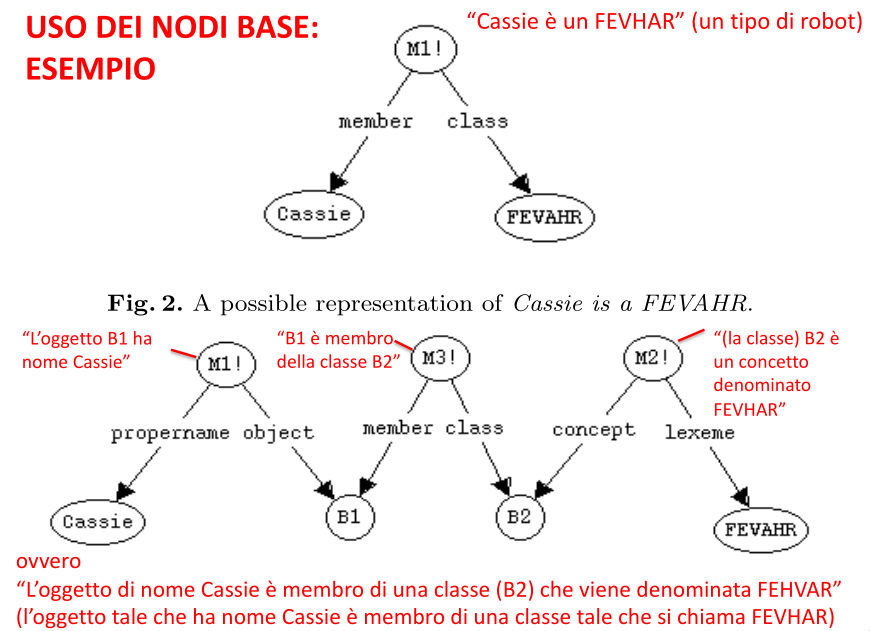
\includegraphics[scale=0.45]{01/nodi di base.png}
\end{center}

}

\subsection{Interrogare la Rete}

\dfn{Find}{
  Il comando utente \newfancyglitter{find} trova uno o più nodi nella rete.
}

\nt{In pratica, la rete si comporta come un database di fatti che può essere
interrogato descrivendo il tipo di fatti cercato.}

\ex{Find}{
\begin{center}
  (find class elephant)
\end{center}
Trova tutti i nodi che hanno un arco di tipo classe che esce dal nodo
e punta al nodo elefante, ossia: \textit{trova tutte le proposizioni che esprimo che qualcosa è un
elefante}.
}

\clm{}{}{
  \begin{itemize}
    \item Il comando find permette di specificare uno o più percorsi per
trovare i nodi cercati. 
\item (find (member- class) canary (object- ability) fly): Trova i canarini (membri della classe canarino) che volano (che
hanno l’abilità di volare). 
\item Tutti i nodi che hanno un arco member entrante, collegato
(tramite un nodo intermedio) a un arco class, e un arco object
entrante, collegato (tramite un nodo intermedio) a un arco ability.
  \end{itemize}
}

\subsection{Rappresentazione delle Credenze e Deduzioni}

\begin{center}
  (assert agent John
act believe
object (build object Opus ability fly))
\end{center}

\begin{itemize}
  \item Attenzione: il sistema non crede che Opus possa
volare ma crede che John creda che Opus possa volare. 
\item Con un find si può scoprire cosa il sistema crede
che John creda. 
\end{itemize}

\begin{center}
  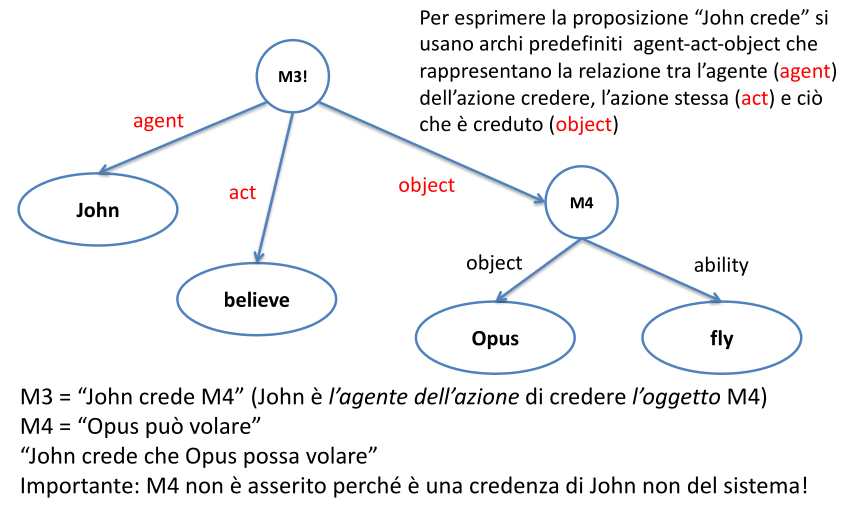
\includegraphics[scale=0.45]{01/john.png}
\end{center}

\dfn{Deduce}{
  Il comando deduce permette di cercare
proposizioni che non sono direttamente
asserite dal sistema ma che il sistema è in
grado di inferire. 
}

\ex{Deduce}{
  \begin{center}
    (deduce member \$x class canary)
  \end{center}
  Trova tutti gli x che appartengono alla classe
dei canarini (\$ indica una variabile).
}

\subsection{Inferenze}

\dfn{Riduzione}{
  La riduzione consiste nel dedurre da un grafo una
porzione contenuta in esso. 
}

\ex{Riduzione}{
  \begin{center}
    (assert agent john act gives object book-1
recipient mary)
  \end{center}
  John dà un libro a Mary. 
  \subsubsection{}
  Può essere ridotto a: 
  \begin{center}
    (deduce agent john act gives object book-1)
  \end{center}
  John dà un libro. 
  \begin{center}
  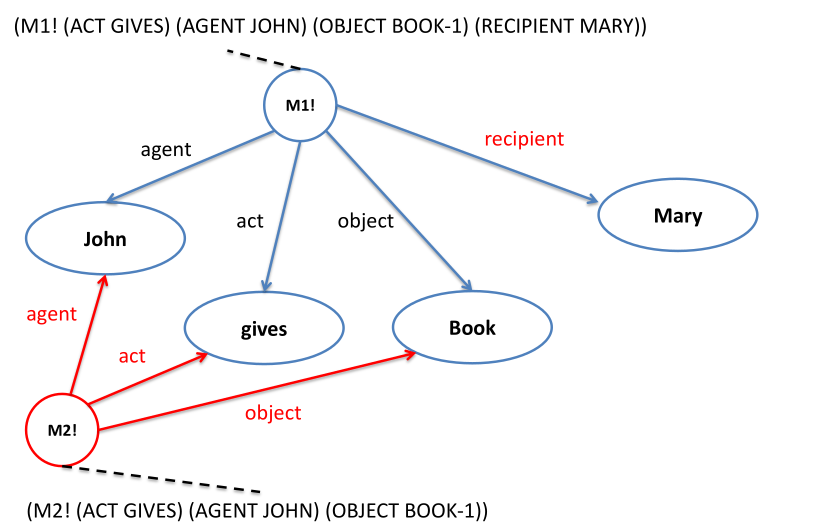
\includegraphics[scale=0.45]{01/book.png}   
  \end{center}
}

\dfn{Define-path}{
  È possibile stabilire che un percorso fatto di certe
relazioni è uguale a una relazione. Si usa il comando define-path.
}

\cor{Compose}{
  Per definire un percorso si usa il comando compose
che si può pensare come comporre una nuova
relazione (arco) basandosi su un percorso di relazioni.
}

\nt{In pratica, si dice che un certo percorso (o meglio ogni
percorso con certe caratteristiche) è uguale a un singolo
arco.}

\ex{Relazione isa transitiva}{
  \begin{center}
    (define-path isa (compose isa
(kstar (compose object- isa))))
  \end{center}
  \begin{itemize}
    \item kstar\footnote{Kleene star per chi si ricorda di LFT.} significa "zero o più occorrenze".
    \item Si legge: isa è guale a isa composto con un percorso di zero o più percorsi
ottenuti da un object- composto con un isa. 
  \end{itemize}
}

\dfn{Regole di Ragionamento}{
  Le regole sono definite dall’utente in modo arbitrario. Fanno parte della base di conoscenza. 
  Permettono di aumentare drasticamente la conoscenza
contenuta nella rete, perché aggiungono nuove
proposizioni non implicite nella rete.
}

\ex{Regole}{
  \begin{center}
  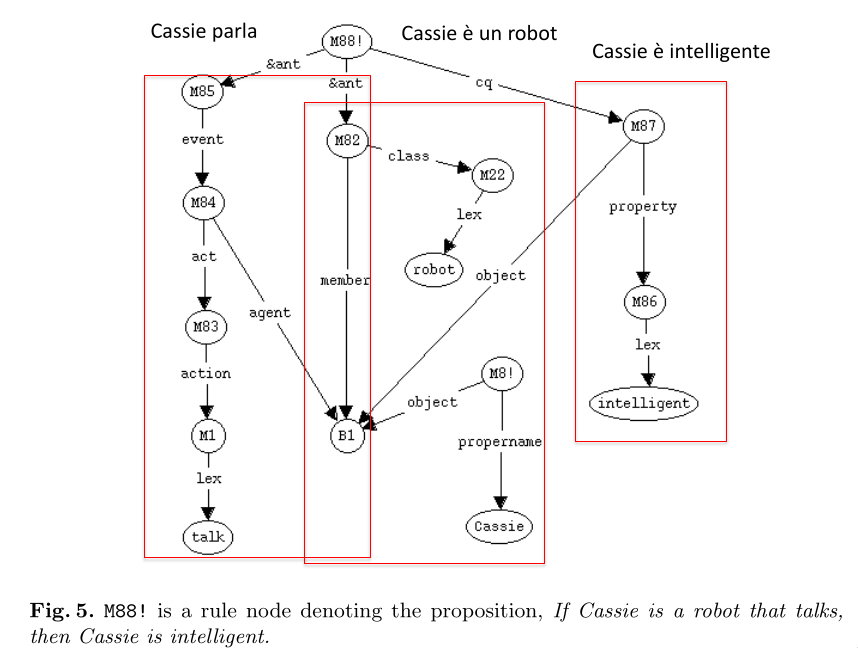
\includegraphics[scale=0.45]{01/regole.png}     
  \end{center}
  \begin{itemize}
\item Antecedente 1 (M85), Cassie parla: in un evento (M84)
B1 è l’agente dell’esecuzione (act) dell’azione (M83)
denominata parlare (lex talk). 
\item Antecedente 2 (M82), Cassie è un robot: B1 è membro
della classe (M22) denominata (lex) robot e ha come
nome proprio (propername) Cassie (quest’ultimo fatto
è asserito). 
\item Conseguente (M87), Cassie è intelligente: B1 (Cassie)
ha la proprietà (M86) di essere intelligente
(denominate “intelligent”).
  \end{itemize}
}

\section{RDF}

\dfn{RDF}{
  RDF è un formato che permette di descrivere risorse.
Una risorsa può essere qualsiasi cosa: un documento, una persona, un
oggetto fisico, un concetto astratto.
}

\dfn{RDFS}{
  RDFS: permette di descrivere relazioni tra risorse. È un linguaggio “property-centric” ed è un'estensione di RDF.
}

\dfn{OWL}{
  OWL (Ontology Web Language): permette di descrivere ontologie computazionali. Si colloca a un livello superiore di RDF. Permette di descrivere relazioni ricche e complesse tra entità
(“complex knowledge about things, groups of things, and relations
between things”).
}

\subsection{Introduzione}

\paragraph{Carta d'Identità di RDF:}

\begin{itemize}
  \item Nato per \fancyglitter{descrivere} risorse
digitali. 
\item Il suo data model è basato sul
  concetto di \fancyglitter{grafo}. 
\item I \fancyglitter{nodi} rappresentano entità e
  gli \fancyglitter{archi} relazioni tra di esse. 
\item Possiede diverse
\fancyglitter{serializzazioni}.
\end{itemize}

\paragraph{Elementi del data model di RDF:}

\begin{itemize}
  \item Triple (organizzate in grafi). 
  \item IRI. 
  \item Letterali. 
  \item Blank nodes. 
  \item Grafi.
\end{itemize}

\nt{L’unità di base di RDF è una tripla, composta di soggetto, predicato e
oggetto. Il soggetto e oggetto possono essere IRI o blank nodes, l’oggetto
può essere anche un letterale, il predicato può essere solo un IRI.}

\dfn{Triple}{
  RDF è formato di triple, che hanno la forma:
Soggetto – Predicato – Oggetto
}

\ex{Triple}{
  \begin{center}
  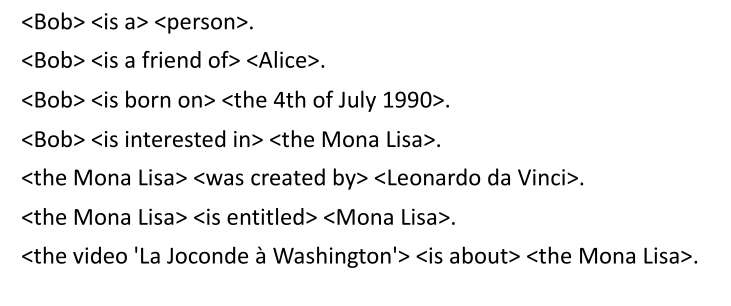
\includegraphics[scale=0.45]{01/t.png}     
  \end{center}
}

\ex{Dalla tripla al grafo}{
  \begin{center}
  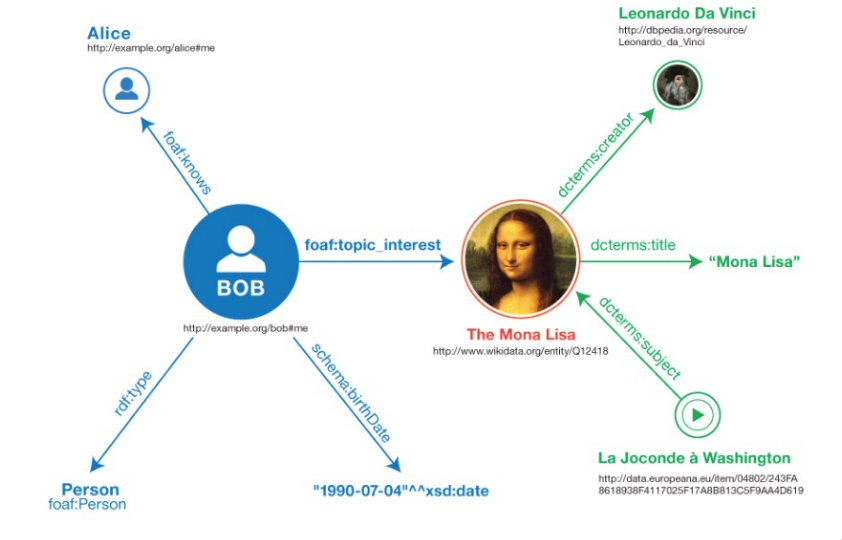
\includegraphics[scale=0.45]{01/t2.png}     
  \end{center}
}

\nt{Gli elementi della tripla devono essere riconducibili
a entità presenti nel web.}

\dfn{URI e IRI}{
  Lo strumento scelto da RDF per rappresentare le
entità è dato dal sistema degli IRI (URI Internazionalizzato).
}

\nt{Cosa rappresenti nella realtà un determinato IRI non è
rilevante: l’importante è che sia de-referenziabile. 

Il predicato è sempre rappresentato da un IRI. }

\dfn{Letterali}{
  Qualsiasi tipo di dato che non sia un IRI (stringhe, numeri, booleani, etc.)
}

\nt{Solo in posizione di oggetto nella tripla. Sostanzialmente coincidono con i data types di XML
Schema, anche se il supporto può essere parziale in
alcuni software.}

\dfn{Blank Node}{Permettono di denotare risorse senza utilizzare un IRI.}

\nt{Un blank node è come una variabile e può comparire in
posizione di soggetto e oggetto nella tripla. Possono essere associati a un identificativo nella
rappresentazione delle triple in un determinato store, ma
non hanno significato al di fuori di esso.}

\subsection{Vocabolari e Grafi}

\dfn{Vocabolari Condivisi}{
  Per descrivere una certa entità, la tripla si basa sull’utilizzo di vocabolari
condivisi. Invece di "inventare" ogni volta i termini per descrivere le entità di cui parla la tripla, meglio usare tutti gli stessi termini.
}

\ex{Utilizzo di vocabolari condivisi}{
    <Bob><http://www.my\_vocab\#like><The Mona Lisa>.

<Bob><http://www.likesanddislikes/loves/adores><The Mona Lisa>.

Questo causa confusione, meglio concordare in anticipo su un unico termine:
<Bob><http://xmlns.com/foaf/0.1/topic\_interest ><The Mona Lisa>.

}


\clm{}{}{
  \begin{itemize}
    \item In molte serializzazioni di RDF, il vocabolario è
identificato da un prefisso, che corrisponde a un
namespace. 
\item RDF non permette di specificare il
significato dei predicati che
mettono in relazione soggetto e
oggetto. 
\item Tuttavia, con RDF si può asserire
che una risorsa appartiene a una
certa tipologia (classe) utilizzando
il predicato type.
  \end{itemize}
}

\dfn{Grafi}{
  Un grafo ha un identificativo dato da un IRI (o un
blank node)
\begin{center}
  Grafo = IRI + triple
\end{center}

}

\cor{Data Set}{
  Un data set RDF è costituito da un insieme di grafi:
  \begin{itemize}
    \item Un grafo anonimo (\fancyglitter{default graph}). 
  \item Zero o più grafi con un nome (\fancyglitter{named graphs}).
  \end{itemize}
}

\section{Turtle}

Storicamente il formato di
serializzazione è stato XML (RDF/XML),
tuttavia XML si è imposto come
standard per la condivisione di
documenti
.
\subsection{Introduzione}

\dfn{Turtle}{
Formato di serializzazione, preferito a RDF/XML per la maggiore
coincisione e leggibilità.
}

\clm{}{}{
\begin{enumerate}
  \item Definizione di prefissi: il "base" diventa il prefisso di default a cui vengono ricondotti tutti gli IRI. 
  \item Commenti: i "cancelletti". 
  \item Triple: espresse secondo certe convenzioni.
\end{enumerate}
}

\begin{figure}[h]
    \centering
    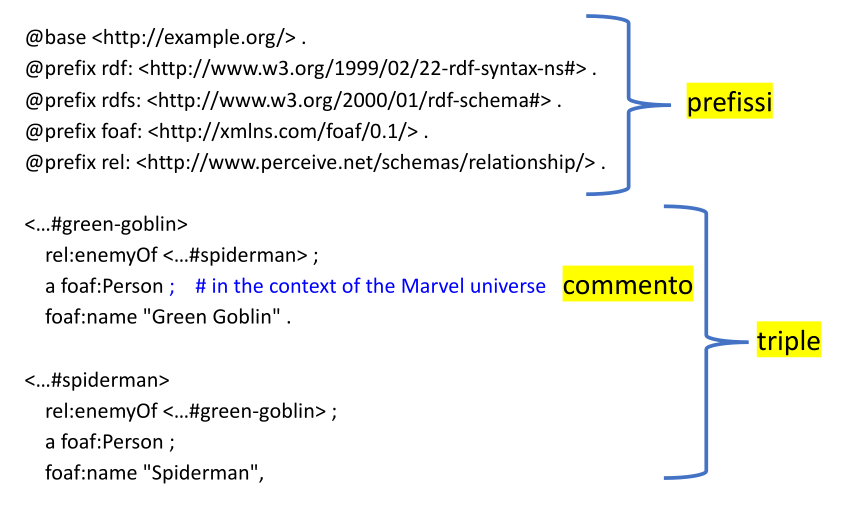
\includegraphics[scale=0.4]{01/turtle.png}
    \caption{Il formato Turtle.}
\end{figure}

\begin{figure}[h]
    \centering
    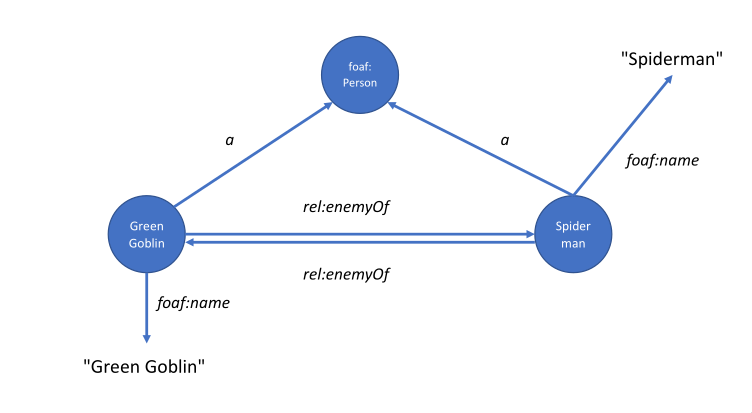
\includegraphics[scale=0.4]{01/turtle2.png}
    \caption{Rappresentazione a grafo.}
\end{figure}

\subsection{Sintassi}

\nt{Gli IRI, se presenti per esteso, sono racchiusi tra $<$ e $>$.
La parte finale che segue \# identifica un frammento (fragment identifier).
}

\dfn{Abbreviazione di Triple}{
“;” indica che allo stesso soggetto si applicano più
predicati (con diverso oggetto), equivale a ripetere il
soggetto.
}

\clm{}{}{
\begin{itemize}
  \item “:”è il prefisso vuoto.
  \item “,” equivale a ripetere soggetto e predicato.
\end{itemize}
}

\nt{
  La sintassi concreta dei blank node in
Turtle è data dalle parentesi quadre $[]$. 

$[]$ da solo indica un soggetto o oggetto
non specificato.

È possibile raggruppare nelle parentesi
un insieme di triple che hanno il blank
node come soggetto.
}

\dfn{Abbreviazione di Valori Numerici}{
  I valori numerici possono essere scritti in modo esteso (forma
lessicale seguita da datatype) oppure in modo abbreviato.
}


\begin{figure}[h]
    \centering
    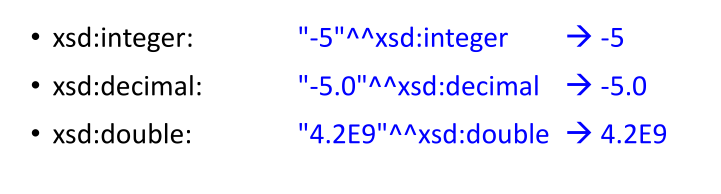
\includegraphics[scale=0.4]{01/numeri.png}
    \caption{Abbreviazioni di numeri.}
\end{figure}

\nt{Lo stesso vale per i booleani (true/false).}

\dfn{N-Triples}{
Sottoinsieme di Turtle senza abbreviazioni e senza
prefissi. Verboso e meno leggibile per la mancanza di
abbreviazioni, ma è migliore per il trasferimento dei data set tra applicazioni. 
}

\nt{N-Quads è la sua estensione che aggiunge alla tripla un
quarto elemento, il graph IRI.}
















